\section*{Step 5}

\begin{custombox}[label={box:Q5}]{Step 5}
	For each dataset generate plots like the ones below - to understand the classification boundaries and the overall performance of the classifiers: 

    \begin{figure}[H]
        \centering
        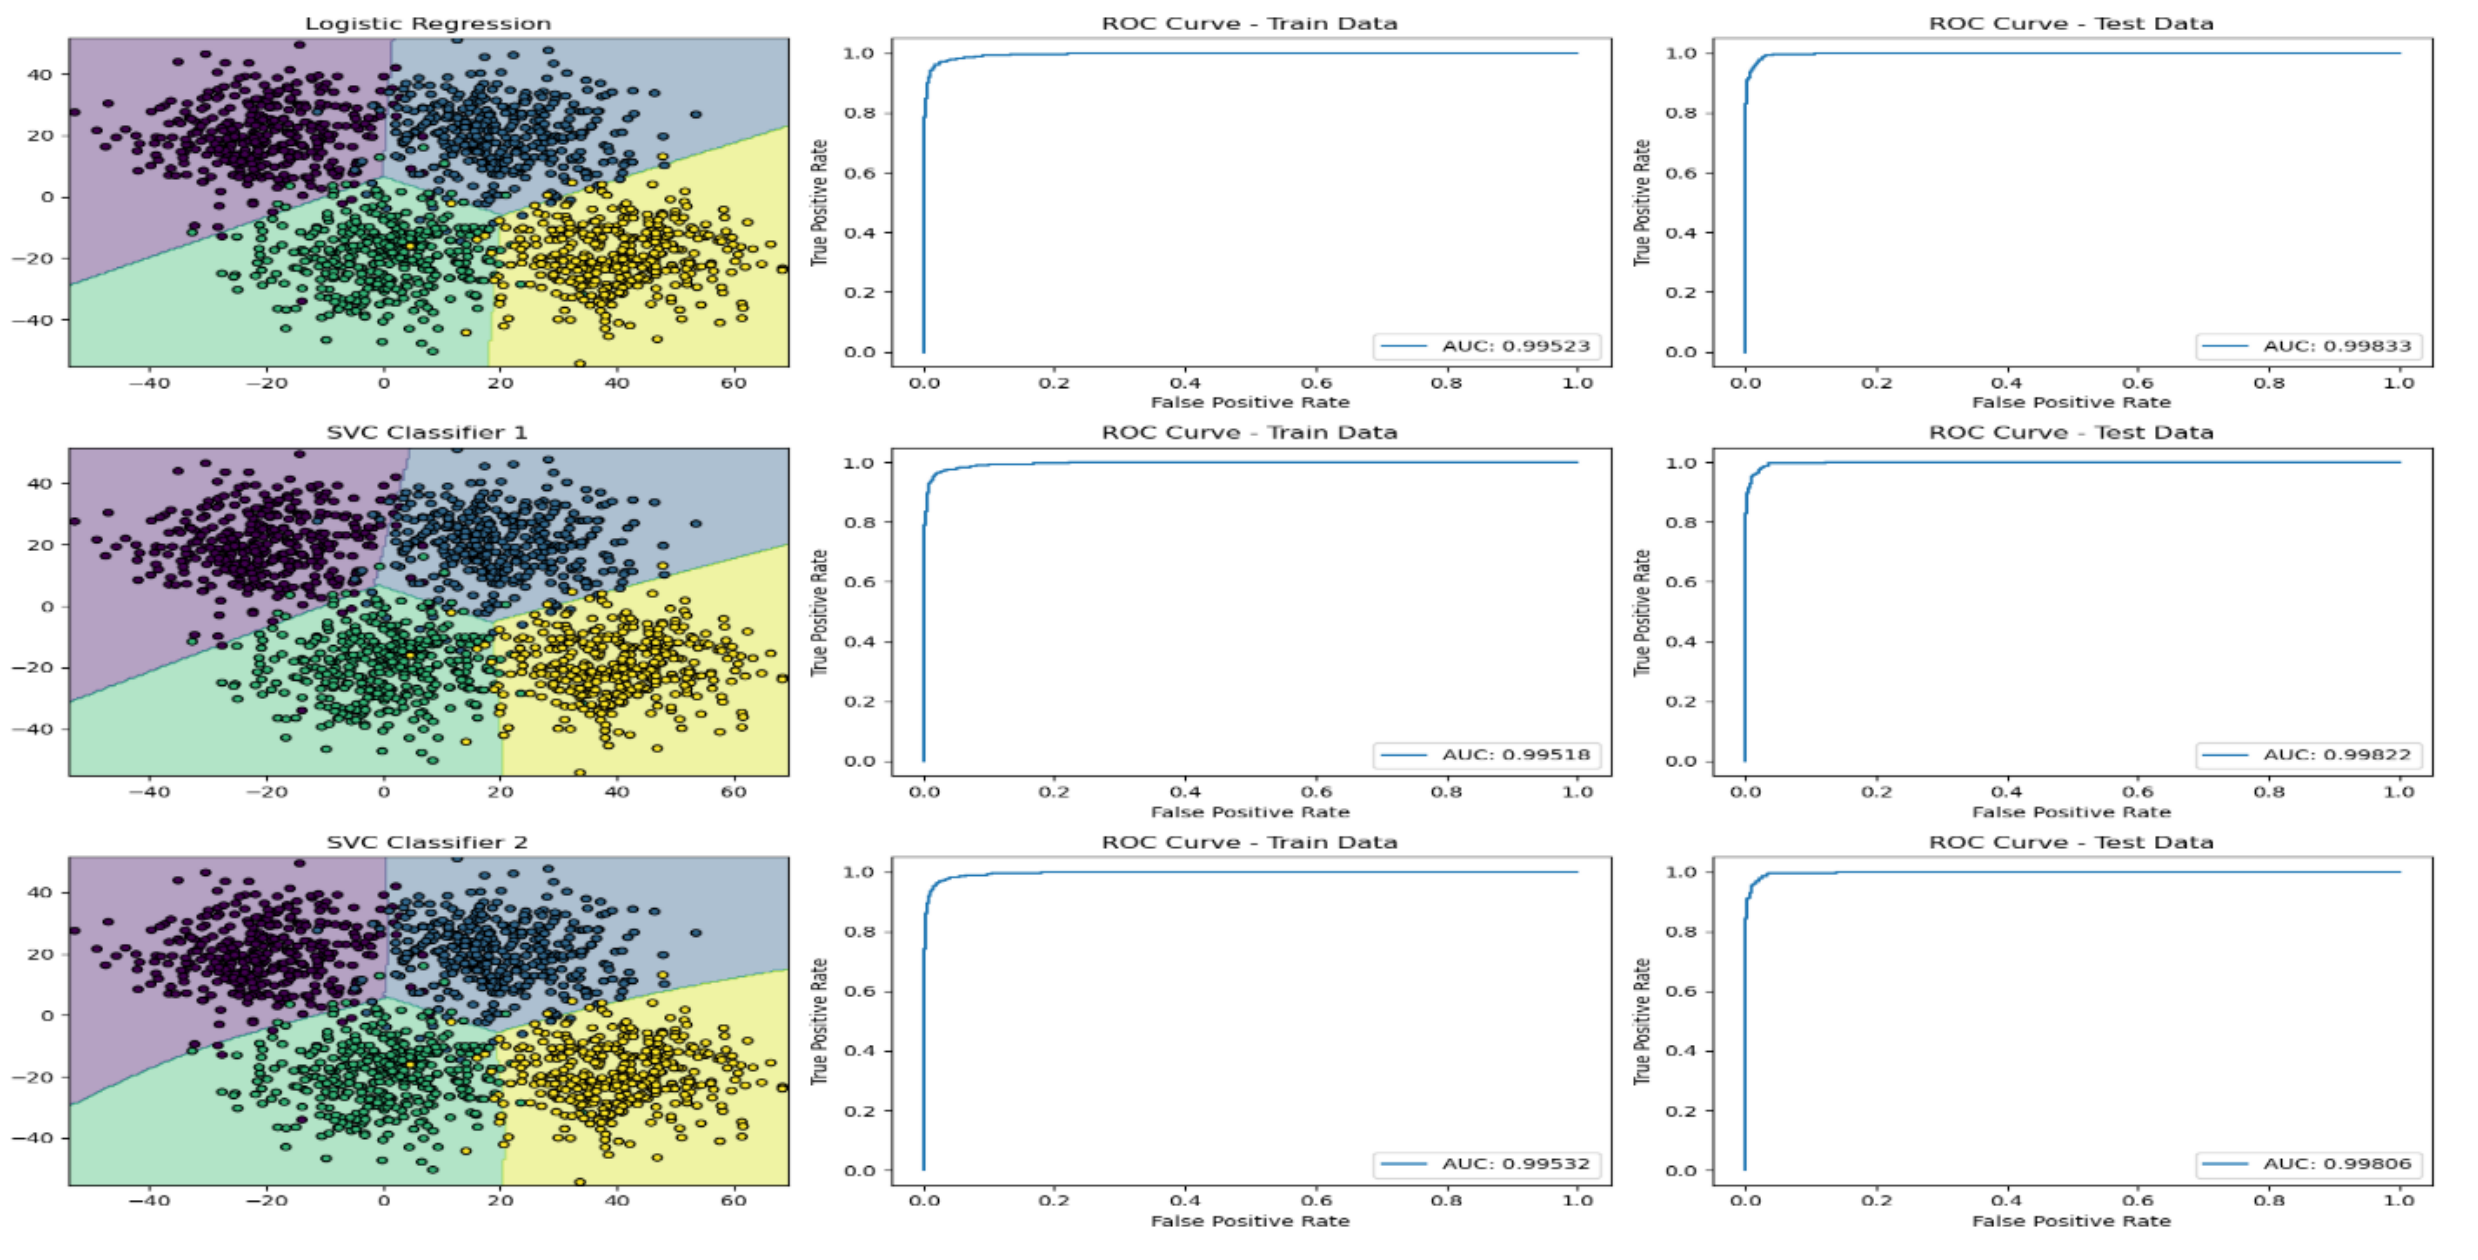
\includegraphics[width=\textwidth]{Images/Step-5-example.png}
        \caption{Example plots for Step 5}
    \end{figure}
\end{custombox}

\vspace{10mm}

For this step, we will generate plots for each dataset to understand the classification boundaries and the overall performance of the classifiers. We will use the \texttt{plot\_decision\_boundary} function to generate these plots. We also plot the ROC Curve for training and testing datasets. The code snippet to generate these plots is shown below:

\begin{lstlisting}[language=Python, caption=Function to draw ROC Curve, label={lst:Q5}]
def draw_roc_curve(model, X, y, label):
    if not isinstance(X, pd.DataFrame):
        X = pd.DataFrame(X, columns=['x1', 'x2'])

    if hasattr(model, 'predict_proba'):
        y_prob = model.predict_proba(X)
    else:
        y_prob = model.decision_function(X)
        y_prob = (y_prob - y_prob.min()) / (y_prob.max() - y_prob.min())

    fpr, tpr, _ = roc_curve(pd.get_dummies(y).values.ravel(), y_prob.ravel())
    auc_score = roc_auc_score(pd.get_dummies(y), y_prob, multi_class='ovr')

    plt.plot(fpr, tpr, label=f'{label} (AUC = {auc_score:.2f})')
    plt.xlabel('False Positive Rate')
    plt.ylabel('True Positive Rate')
    plt.title(f'ROC Curve - {label}')
    plt.legend()
\end{lstlisting}

\clearpage

\begin{lstlisting}[language=Python, caption=Generating Decision Boundaries and ROC Curves, label={lst:Q5.1}]
def draw_plots(classifiers, datasets):
    for i, (data, label) in enumerate(datasets):
        plt.figure(figsize=(18, 15))
        
        for row, (name, clf) in enumerate(classifiers.items()):
            x_train, x_test, y_train, y_test = train_test_split(data[['x1', 'x2']], data['y'], test_size=0.2, random_state=42)
            
            x_train_df = pd.DataFrame(x_train, columns=['x1', 'x2'])
            x_test_df = pd.DataFrame(x_test, columns=['x1', 'x2'])
            y_train = pd.Series(y_train)
            
            clf.fit(x_train_df, y_train.values)

            plt.subplot(len(classifiers)//2, 3, (row % 5) * 3 + 1)
            draw_decision_boundary(clf, x_train_df.values, y_train.values, size=5, edgecolor=None)
            plt.title(f'{name} - {label}')
            plt.xlabel('x1')
            plt.ylabel('x2')

            plt.subplot(len(classifiers)//2, 3, (row % 5) * 3 + 2)
            draw_roc_curve(clf, x_train_df, y_train, 'Train')

            plt.subplot(len(classifiers)//2, 3, (row % 5) * 3 + 3)
            draw_roc_curve(clf, x_test_df, y_test, 'Test')

            if row == 4:
                plt.tight_layout()
                plt.savefig(f'Images/dataset-{i+1}-roc-curves-1.png', dpi=400)
                plt.show()
                plt.figure(figsize=(18, 15))


        plt.tight_layout()
        plt.savefig(f'Images/dataset-{i+1}-roc-curves-2.png', dpi=400)
        plt.show()

draw_plots(classifiers, datasets)
\end{lstlisting}

\begin{definition*}[True Positive Rate \& False Positive Rate]
    The true positive rate (TPR) is the proportion of positive cases that are correctly identified by the classifier. The false positive rate (FPR) is the proportion of negative cases that are incorrectly identified as positive by the classifier. These rates are defined as follows:
    \begin{align*}
        TPR &= \frac{TP}{TP + FN} \\
        FPR &= \frac{FP}{FP + TN}
    \end{align*}
    % where:
    % \begin{itemize}
    %     \item $TP$ is the number of true positives,
    %     \item $FP$ is the number of false positives,
    %     \item $TN$ is the number of true negatives, and
    %     \item $FN$ is the number of false negatives.
    % \end{itemize}
\end{definition*}

\clearpage

\begin{definition*}[ROC Curve]
    The ROC curve is a graphical representation of the true positive rate against the false positive rate for the different possible cutpoints of a diagnostic test. The area under the ROC curve (AUC) is a measure of how well a parameter can distinguish between two diagnostic groups (diseased/normal).

    The ROC curve is a useful tool for a few reasons:
    \begin{itemize}
        \item The ROC curve is invariant to the prevalence of the disease.
        \item The ROC curve is a useful tool to compare the performance of different classifiers.
        \item The ROC curve is a useful tool to determine the optimal threshold for a classifier.
    \end{itemize}
\end{definition*}

% About Good ROC Curves
\begin{definition*}[Good ROC Curves]
    A good ROC curve is one that is close to the top-left corner of the plot. The closer the ROC curve is to the top-left corner, the better the classifier is at distinguishing between the positive and negative classes. A perfect classifier will have an ROC curve that passes through the top-left corner of the plot.

    The area under the ROC curve (AUC) is a measure of how well a parameter can distinguish between two diagnostic groups (diseased/normal). The AUC score ranges from 0 to 1, where 1 indicates a perfect classifier and 0.5 indicates a random classifier.
\end{definition*}

% About Ideal ROC Curves
\begin{definition*}[Ideal ROC Curves]
    An ideal ROC curve is one that passes through the top-left corner of the plot. An ideal ROC curve indicates that the classifier is able to perfectly distinguish between the positive and negative classes. An ideal ROC curve will have an AUC score of 1.
\end{definition*}

We define a function \texttt{draw\_roc\_curve} to draw the ROC curve for the given model, input data, and label. We then define a function \texttt{draw\_plots} to generate the decision boundaries and ROC curves for each dataset using the classifiers defined in Step 4. We iterate over each dataset and classifier to generate the plots. We save the plots as images in the \texttt{Images} directory. The generated plots are shown below:

\clearpage

\begin{figure}[H]
    \centering
    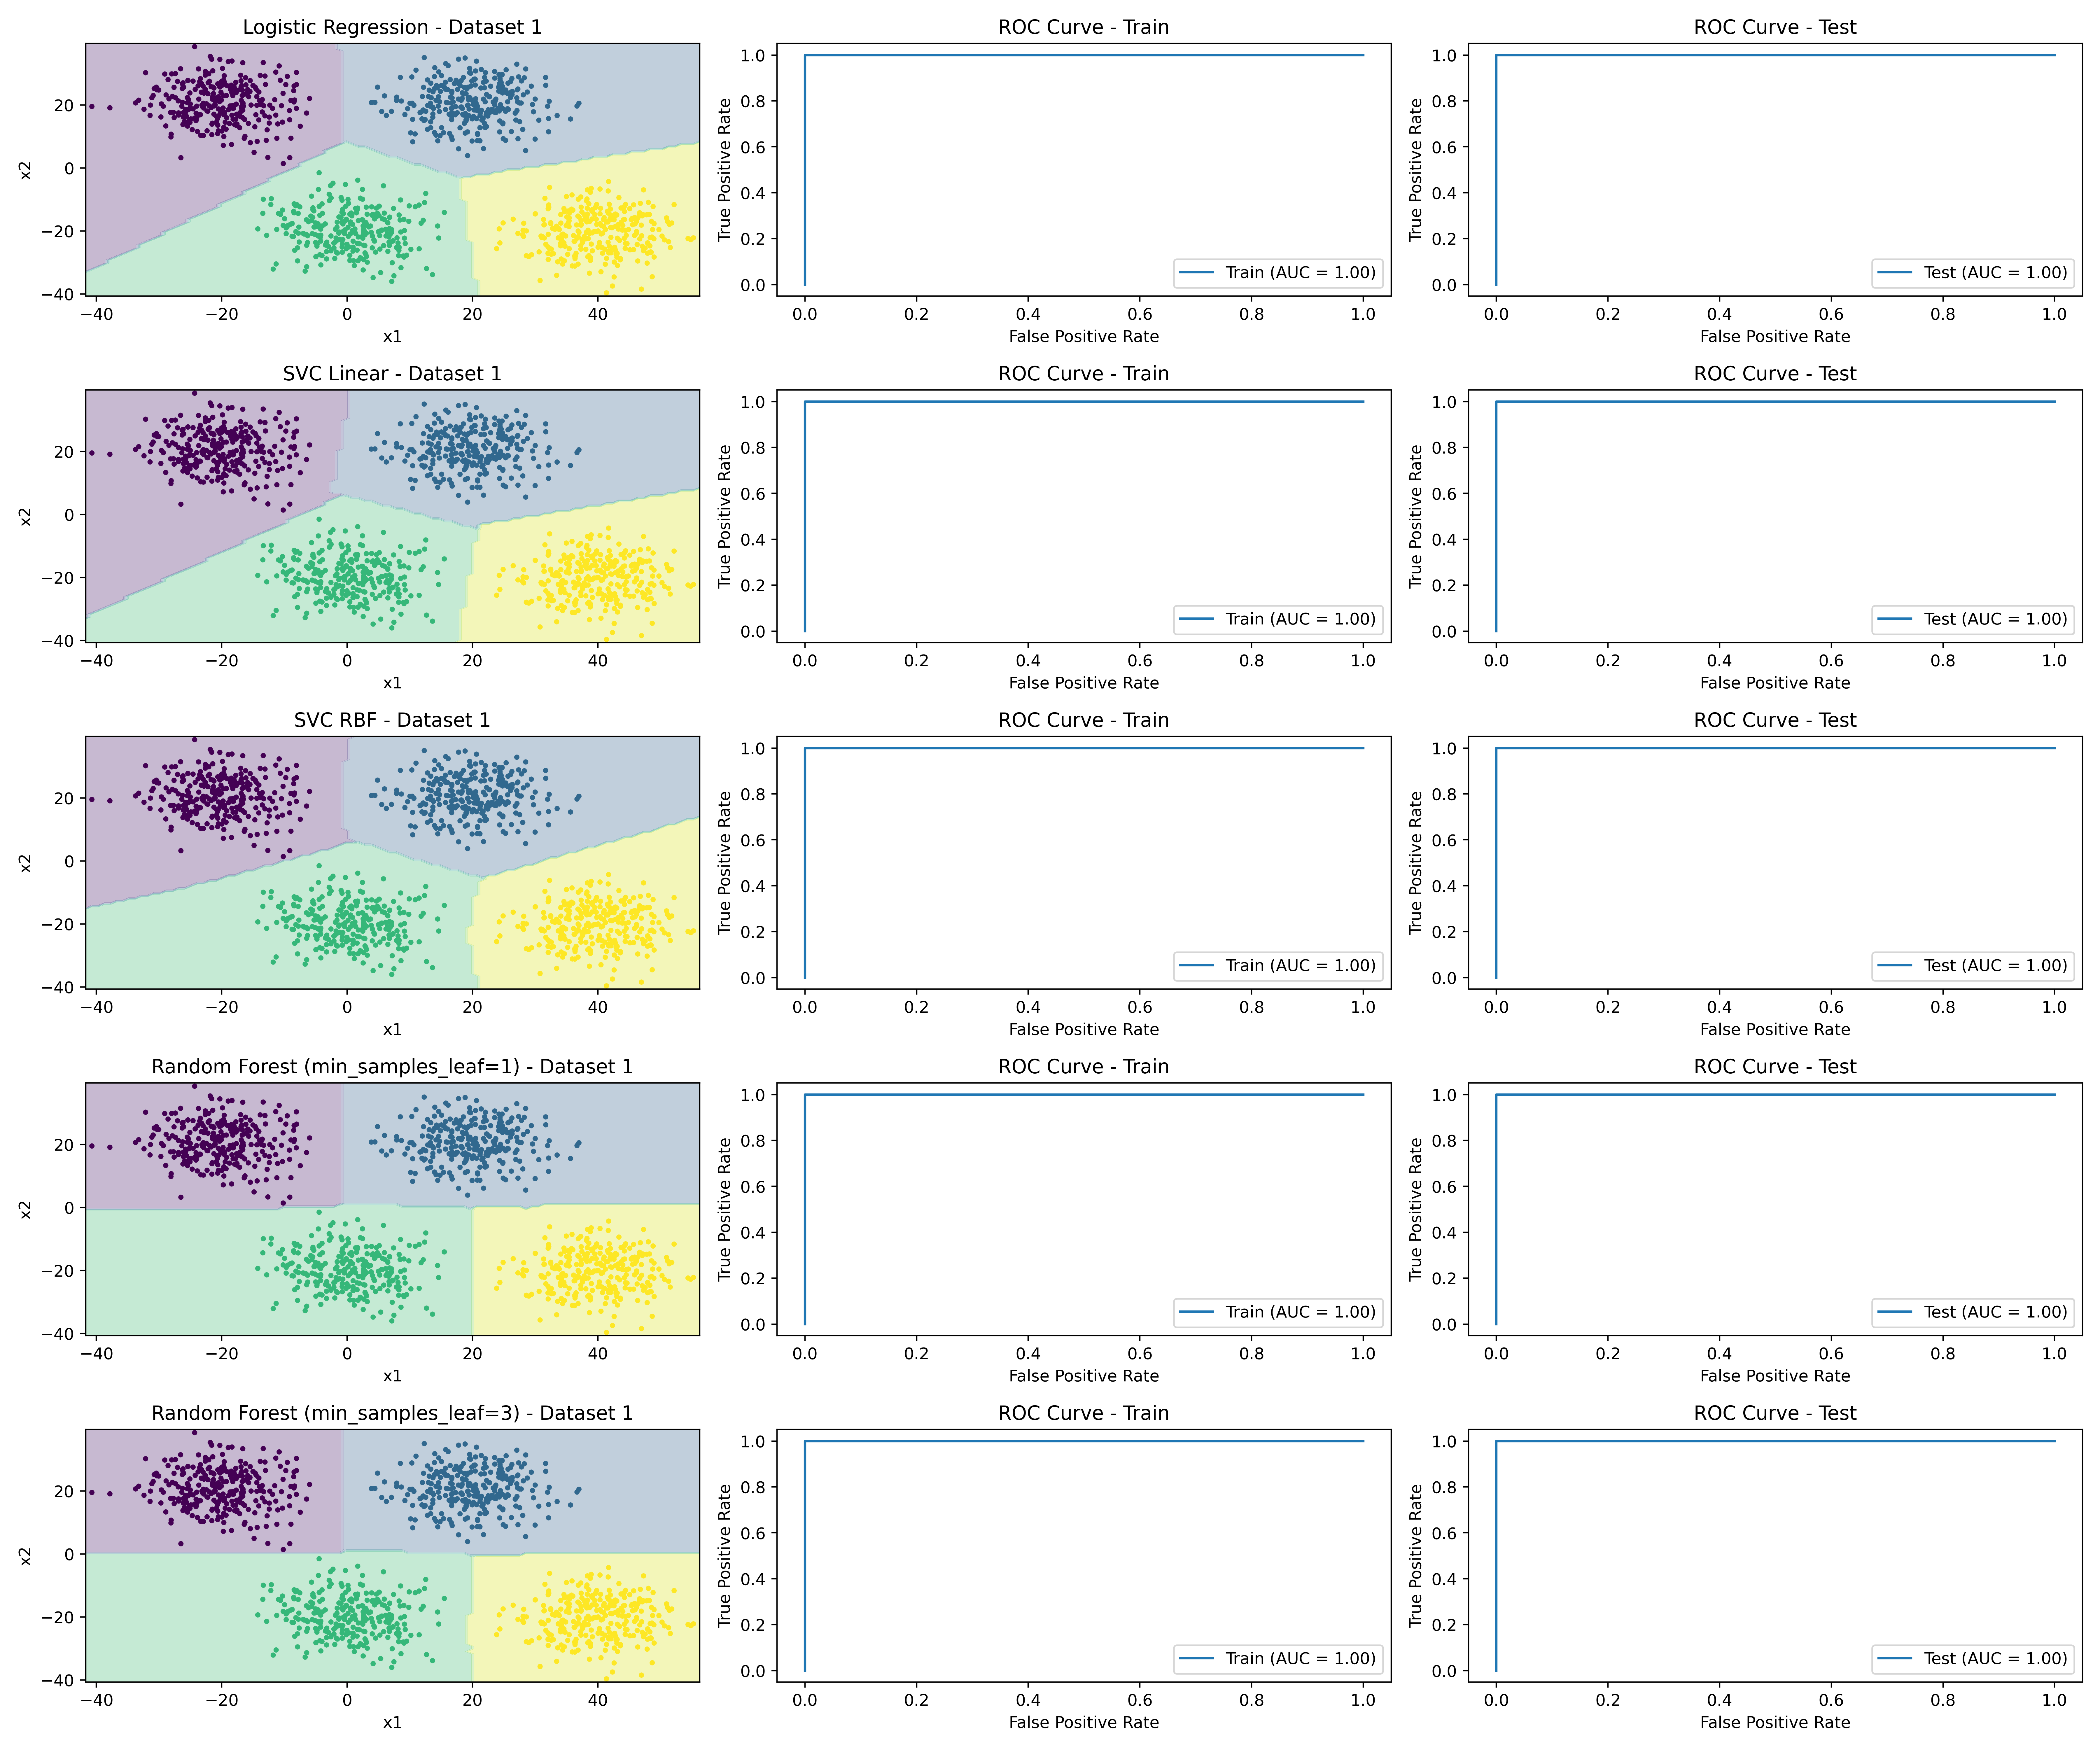
\includegraphics[width=\textwidth]{Images/dataset-1-roc-curves-1.png}
    \caption{ROC Curves for Dataset 1}
\end{figure}

In this set of 5 Classification algorithms for Dataset 1, the Decision Boundaries are plotted for each algorithm. The ROC Curves for the training and testing datasets are also plotted. The ROC Curve for the training dataset is shown in the middle column, and the ROC Curve for the testing dataset is shown in the right column. The AUC score is also displayed in the legend of the ROC Curve.

We observe that the Decision Boundaries are different for each algorithm, but the AUC score for all of them is exactly 1 and the ROC Curves are ideal. This indicates that all the algorithms are able to perfectly classify the data points in Dataset 1.

\begin{figure}[H]
    \centering
    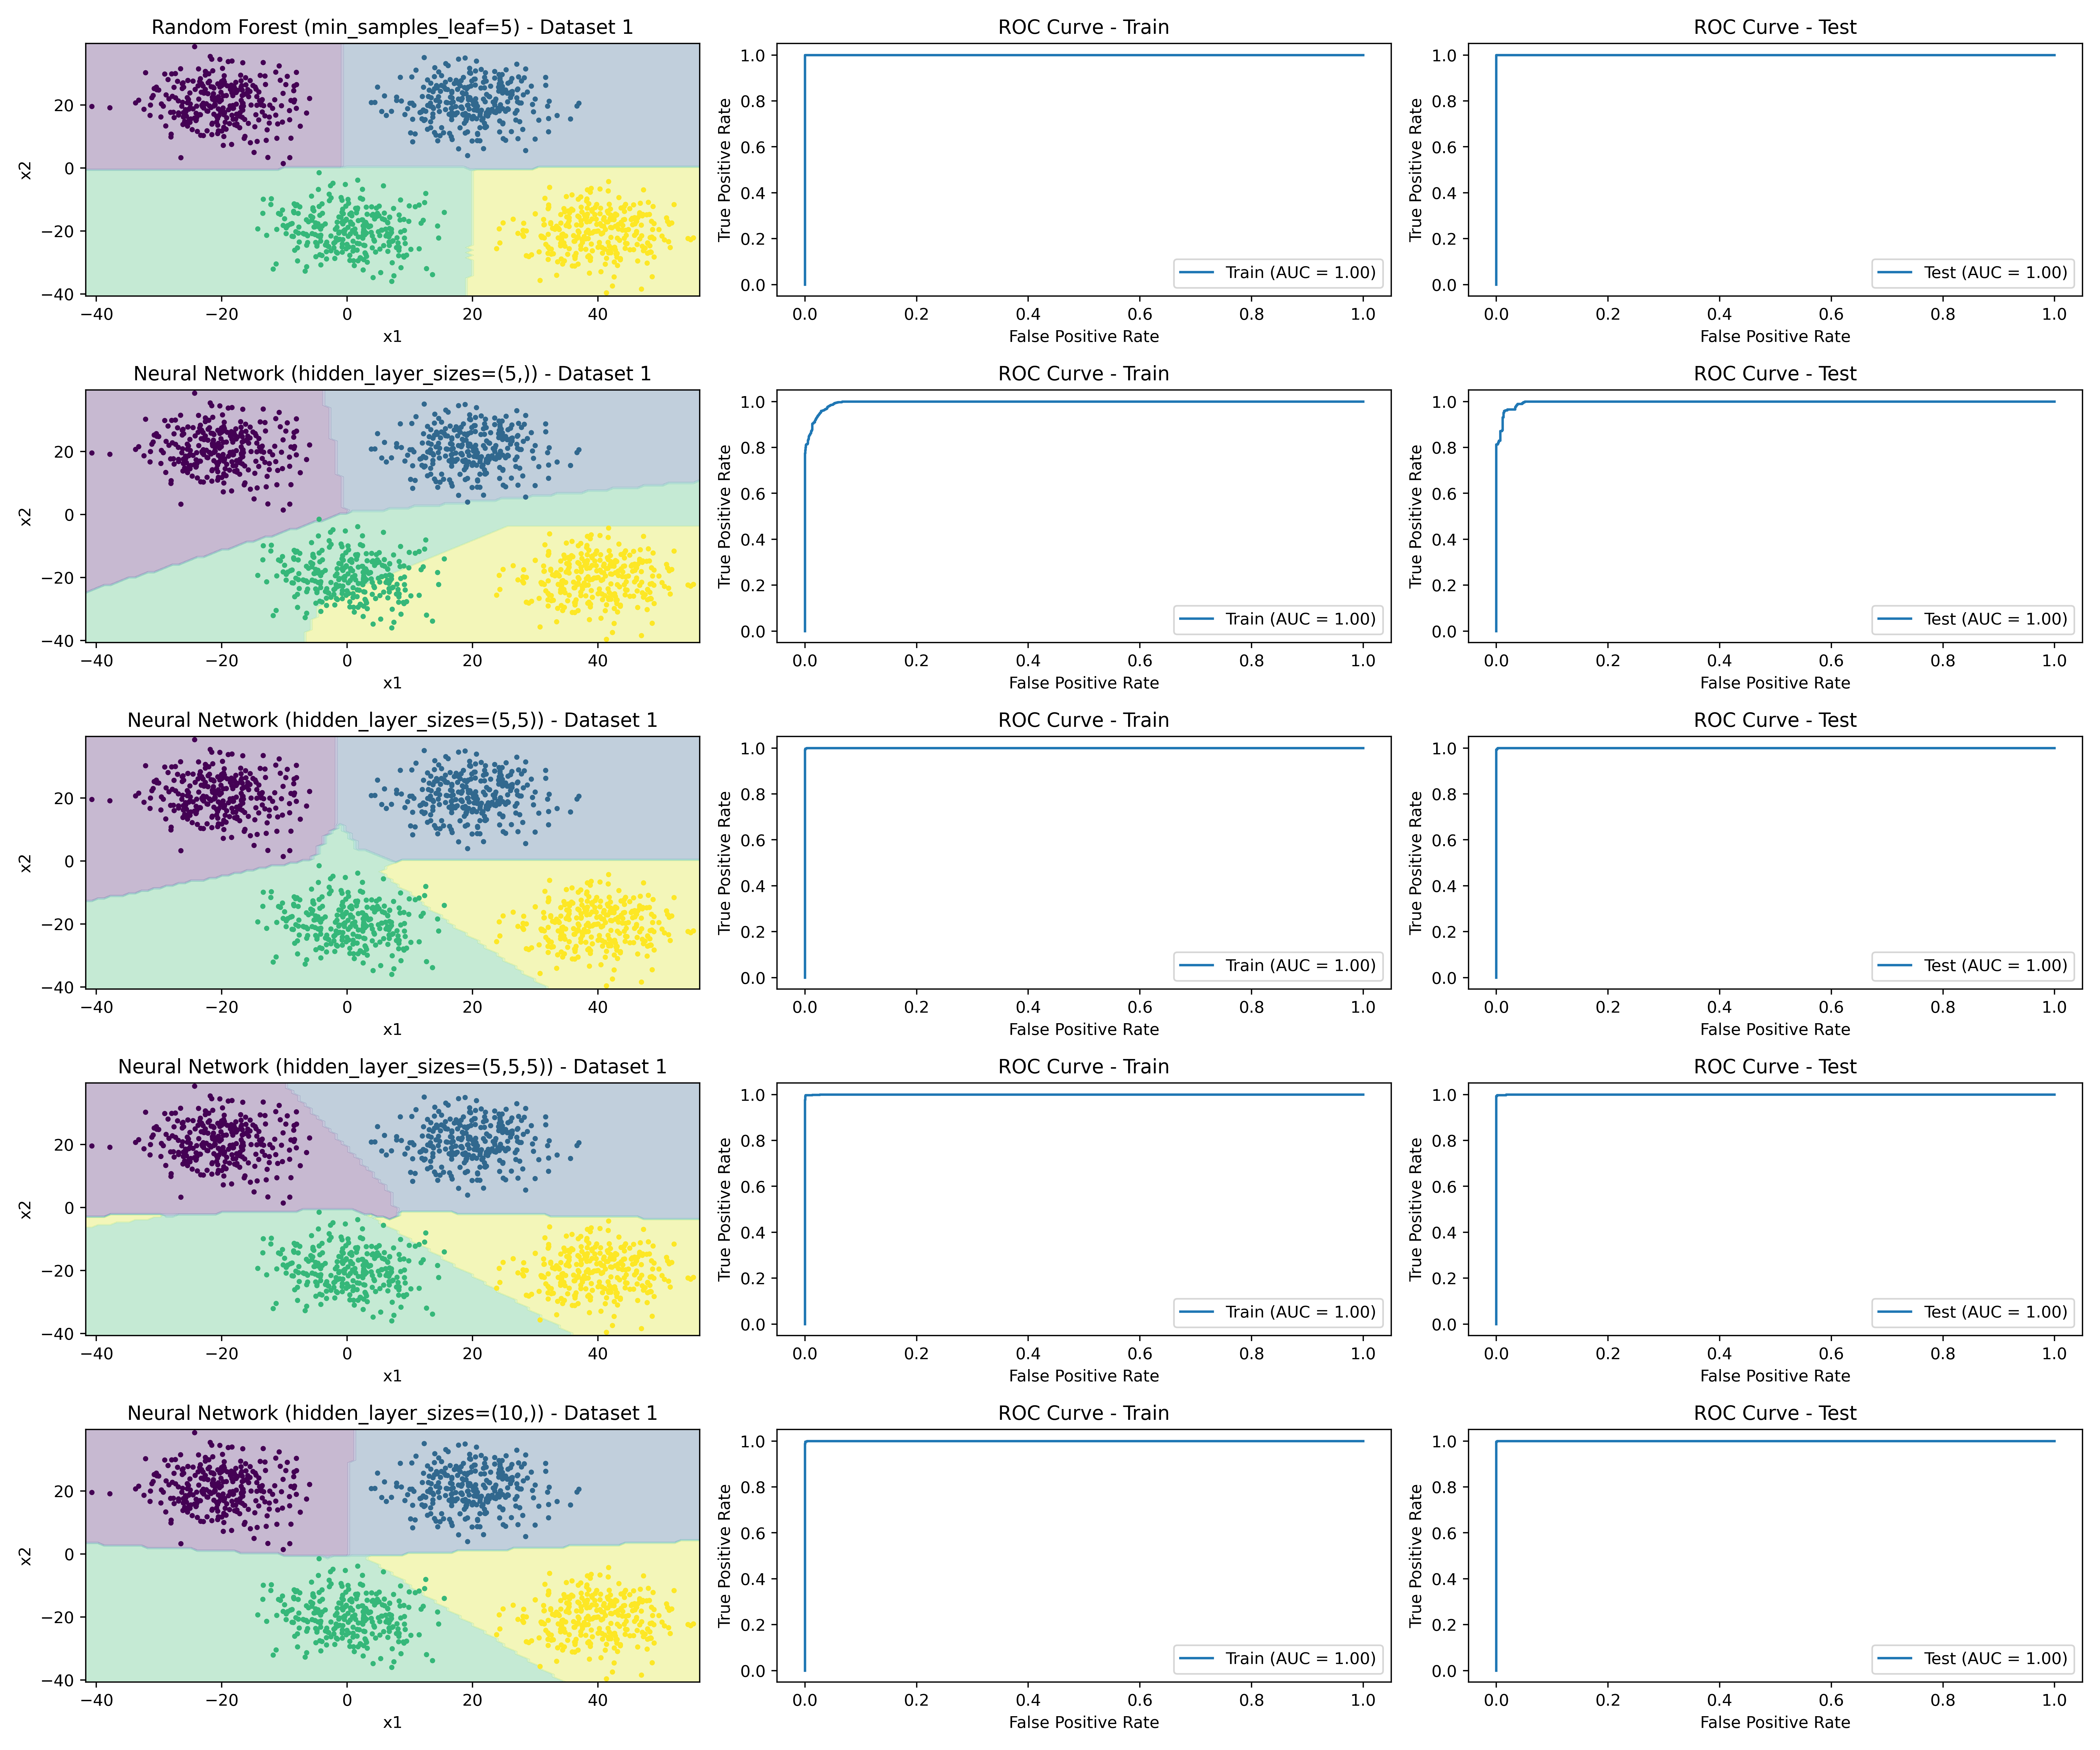
\includegraphics[width=\textwidth]{Images/dataset-1-roc-curves-2.png}
    \caption{ROC Curves for Dataset 1 (continued)}
\end{figure}

Here, we observe that the Decision Boundaries are different for each algorithm, but the AUC score for all of them is exactly 1 and the ROC Curves are almost ideal. This indicates that all the algorithms are able to perfectly classify the data points in Dataset 1. 

\begin{figure}[H]
    \centering
    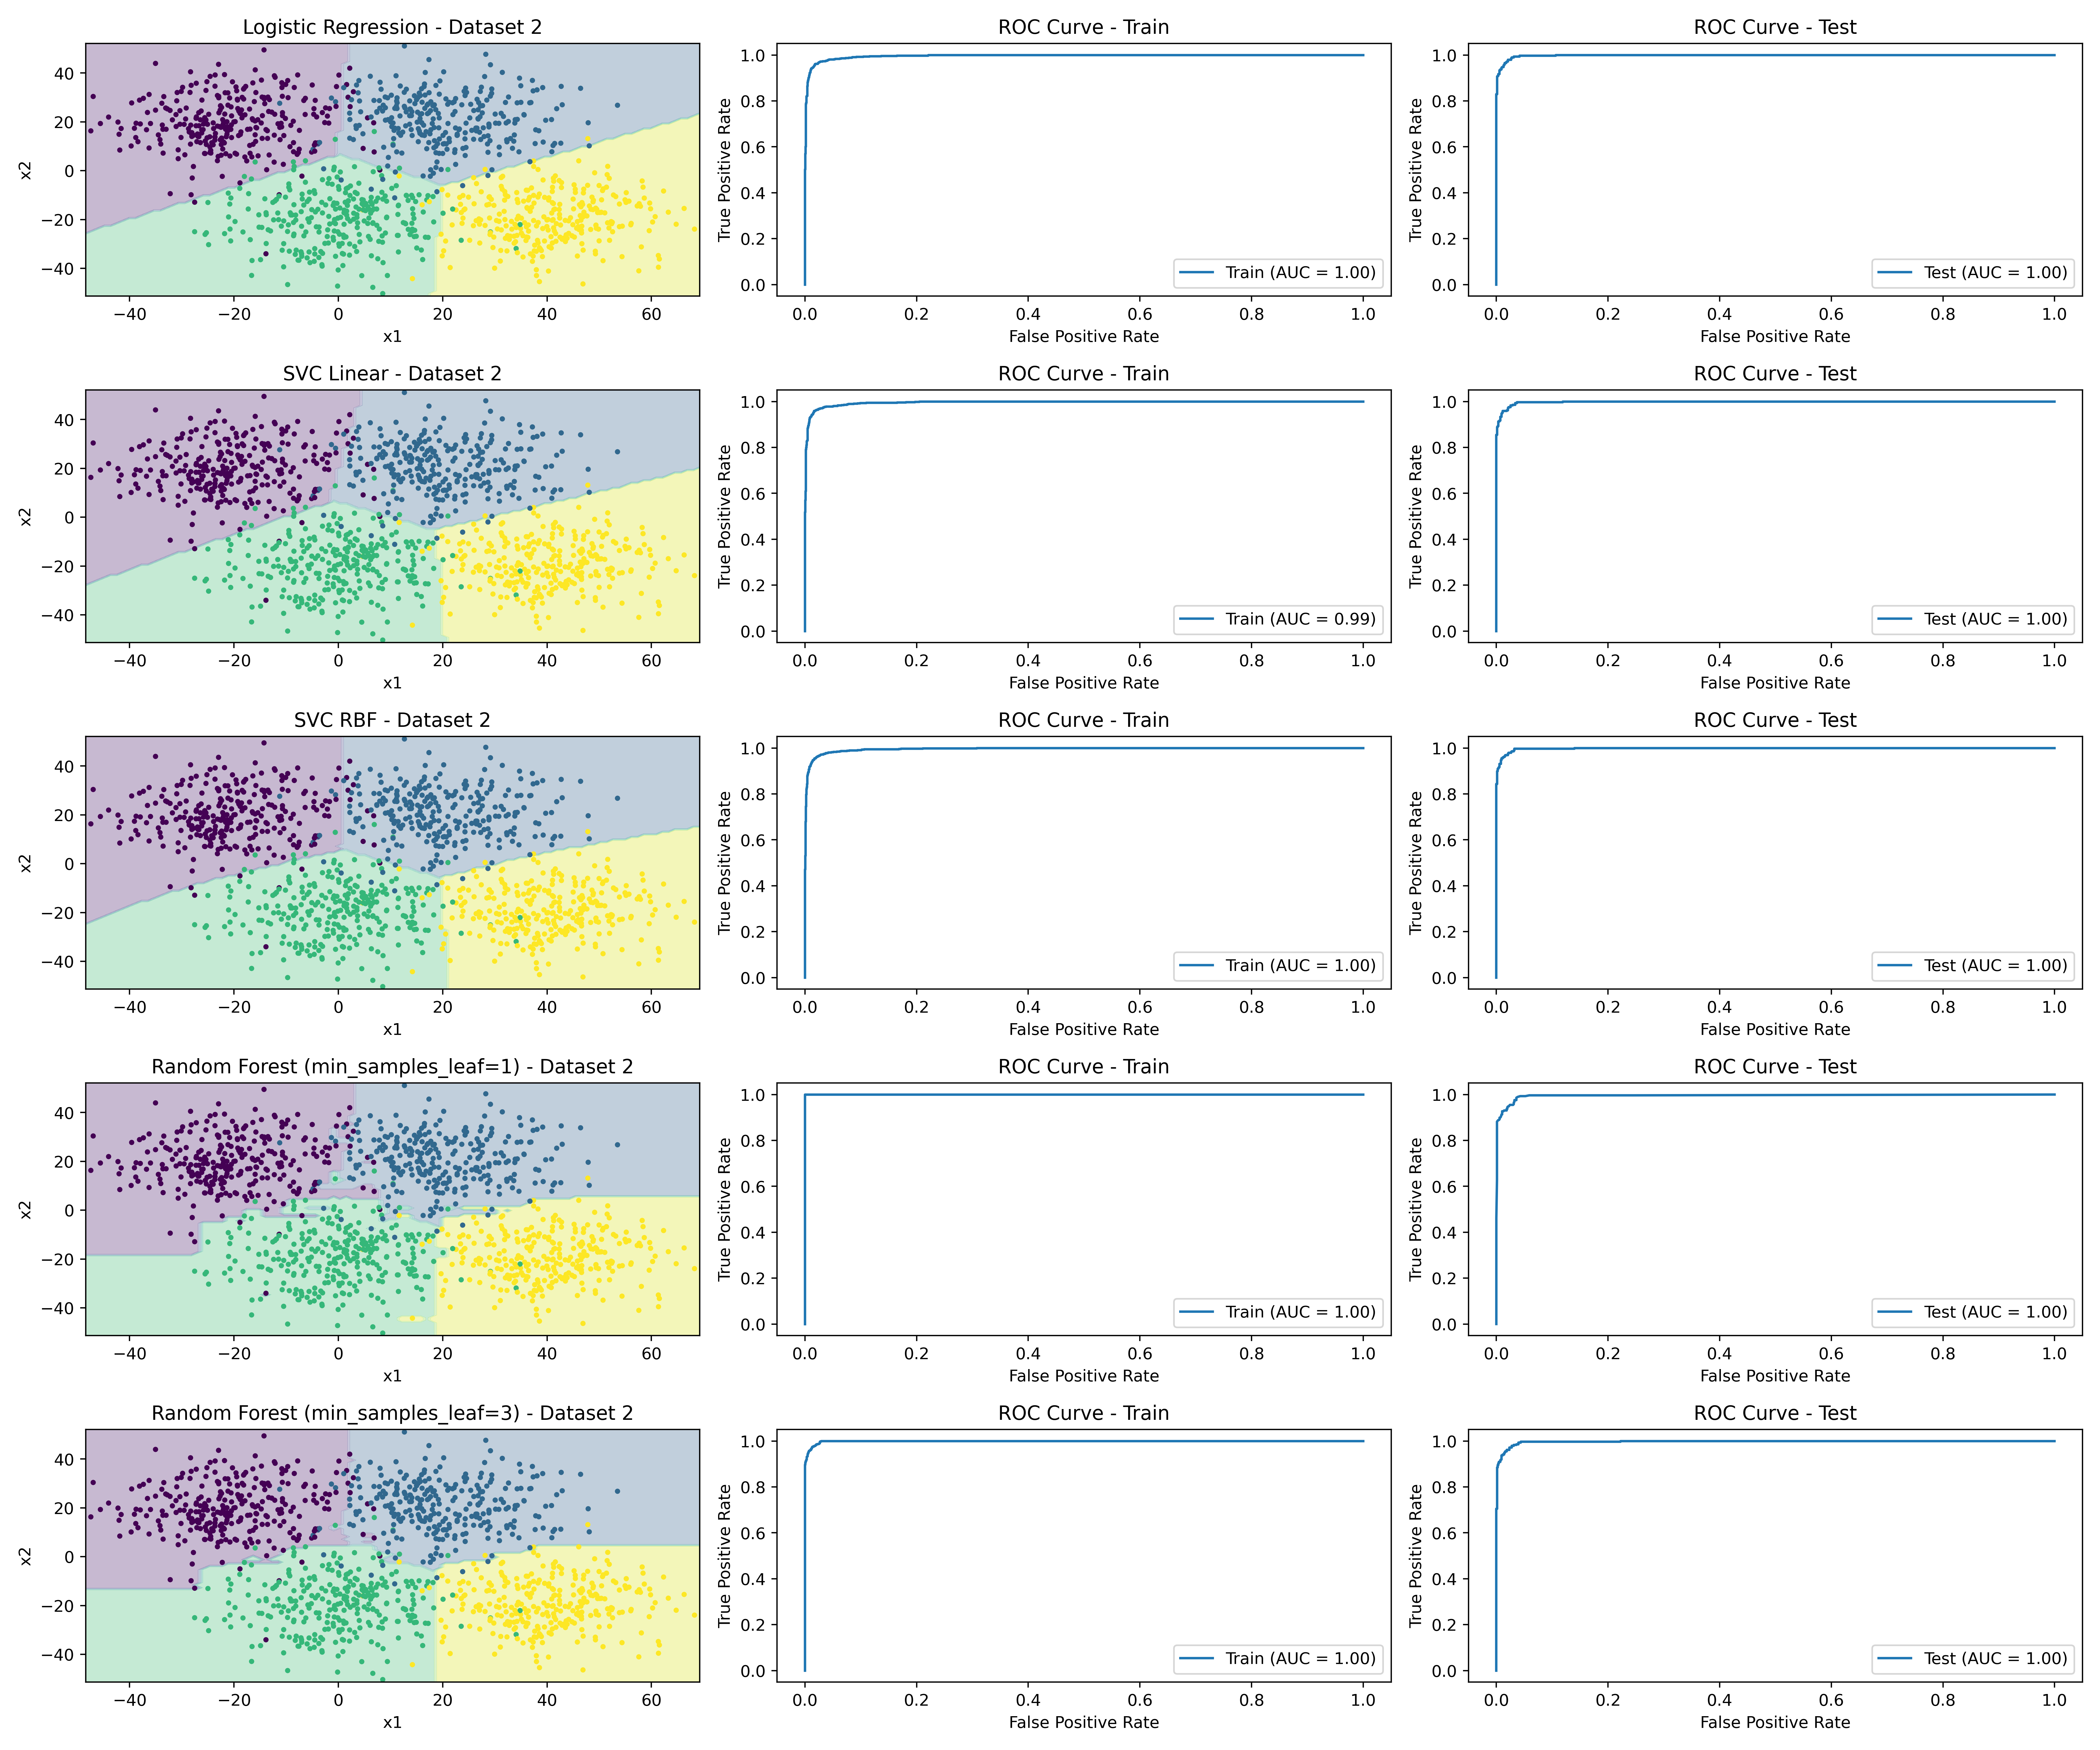
\includegraphics[width=\textwidth]{Images/dataset-2-roc-curves-1.png}
    \caption{ROC Curves for Dataset 2}
\end{figure}

Here, we observe that the Decision Boundaries are different for each algorithm, and the AUC score for all of them are close to 1 but not exactly 1. This indicates that all the algorithms are able to classify the data points in Dataset 2 with high accuracy but not perfectly.

The ROC Curves are also not ideal for all the algorithms, but they are close to the top-left corner of the plot. This indicates that the classifiers are able to distinguish between the positive and negative classes with high accuracy.

\begin{figure}[H]
    \centering
    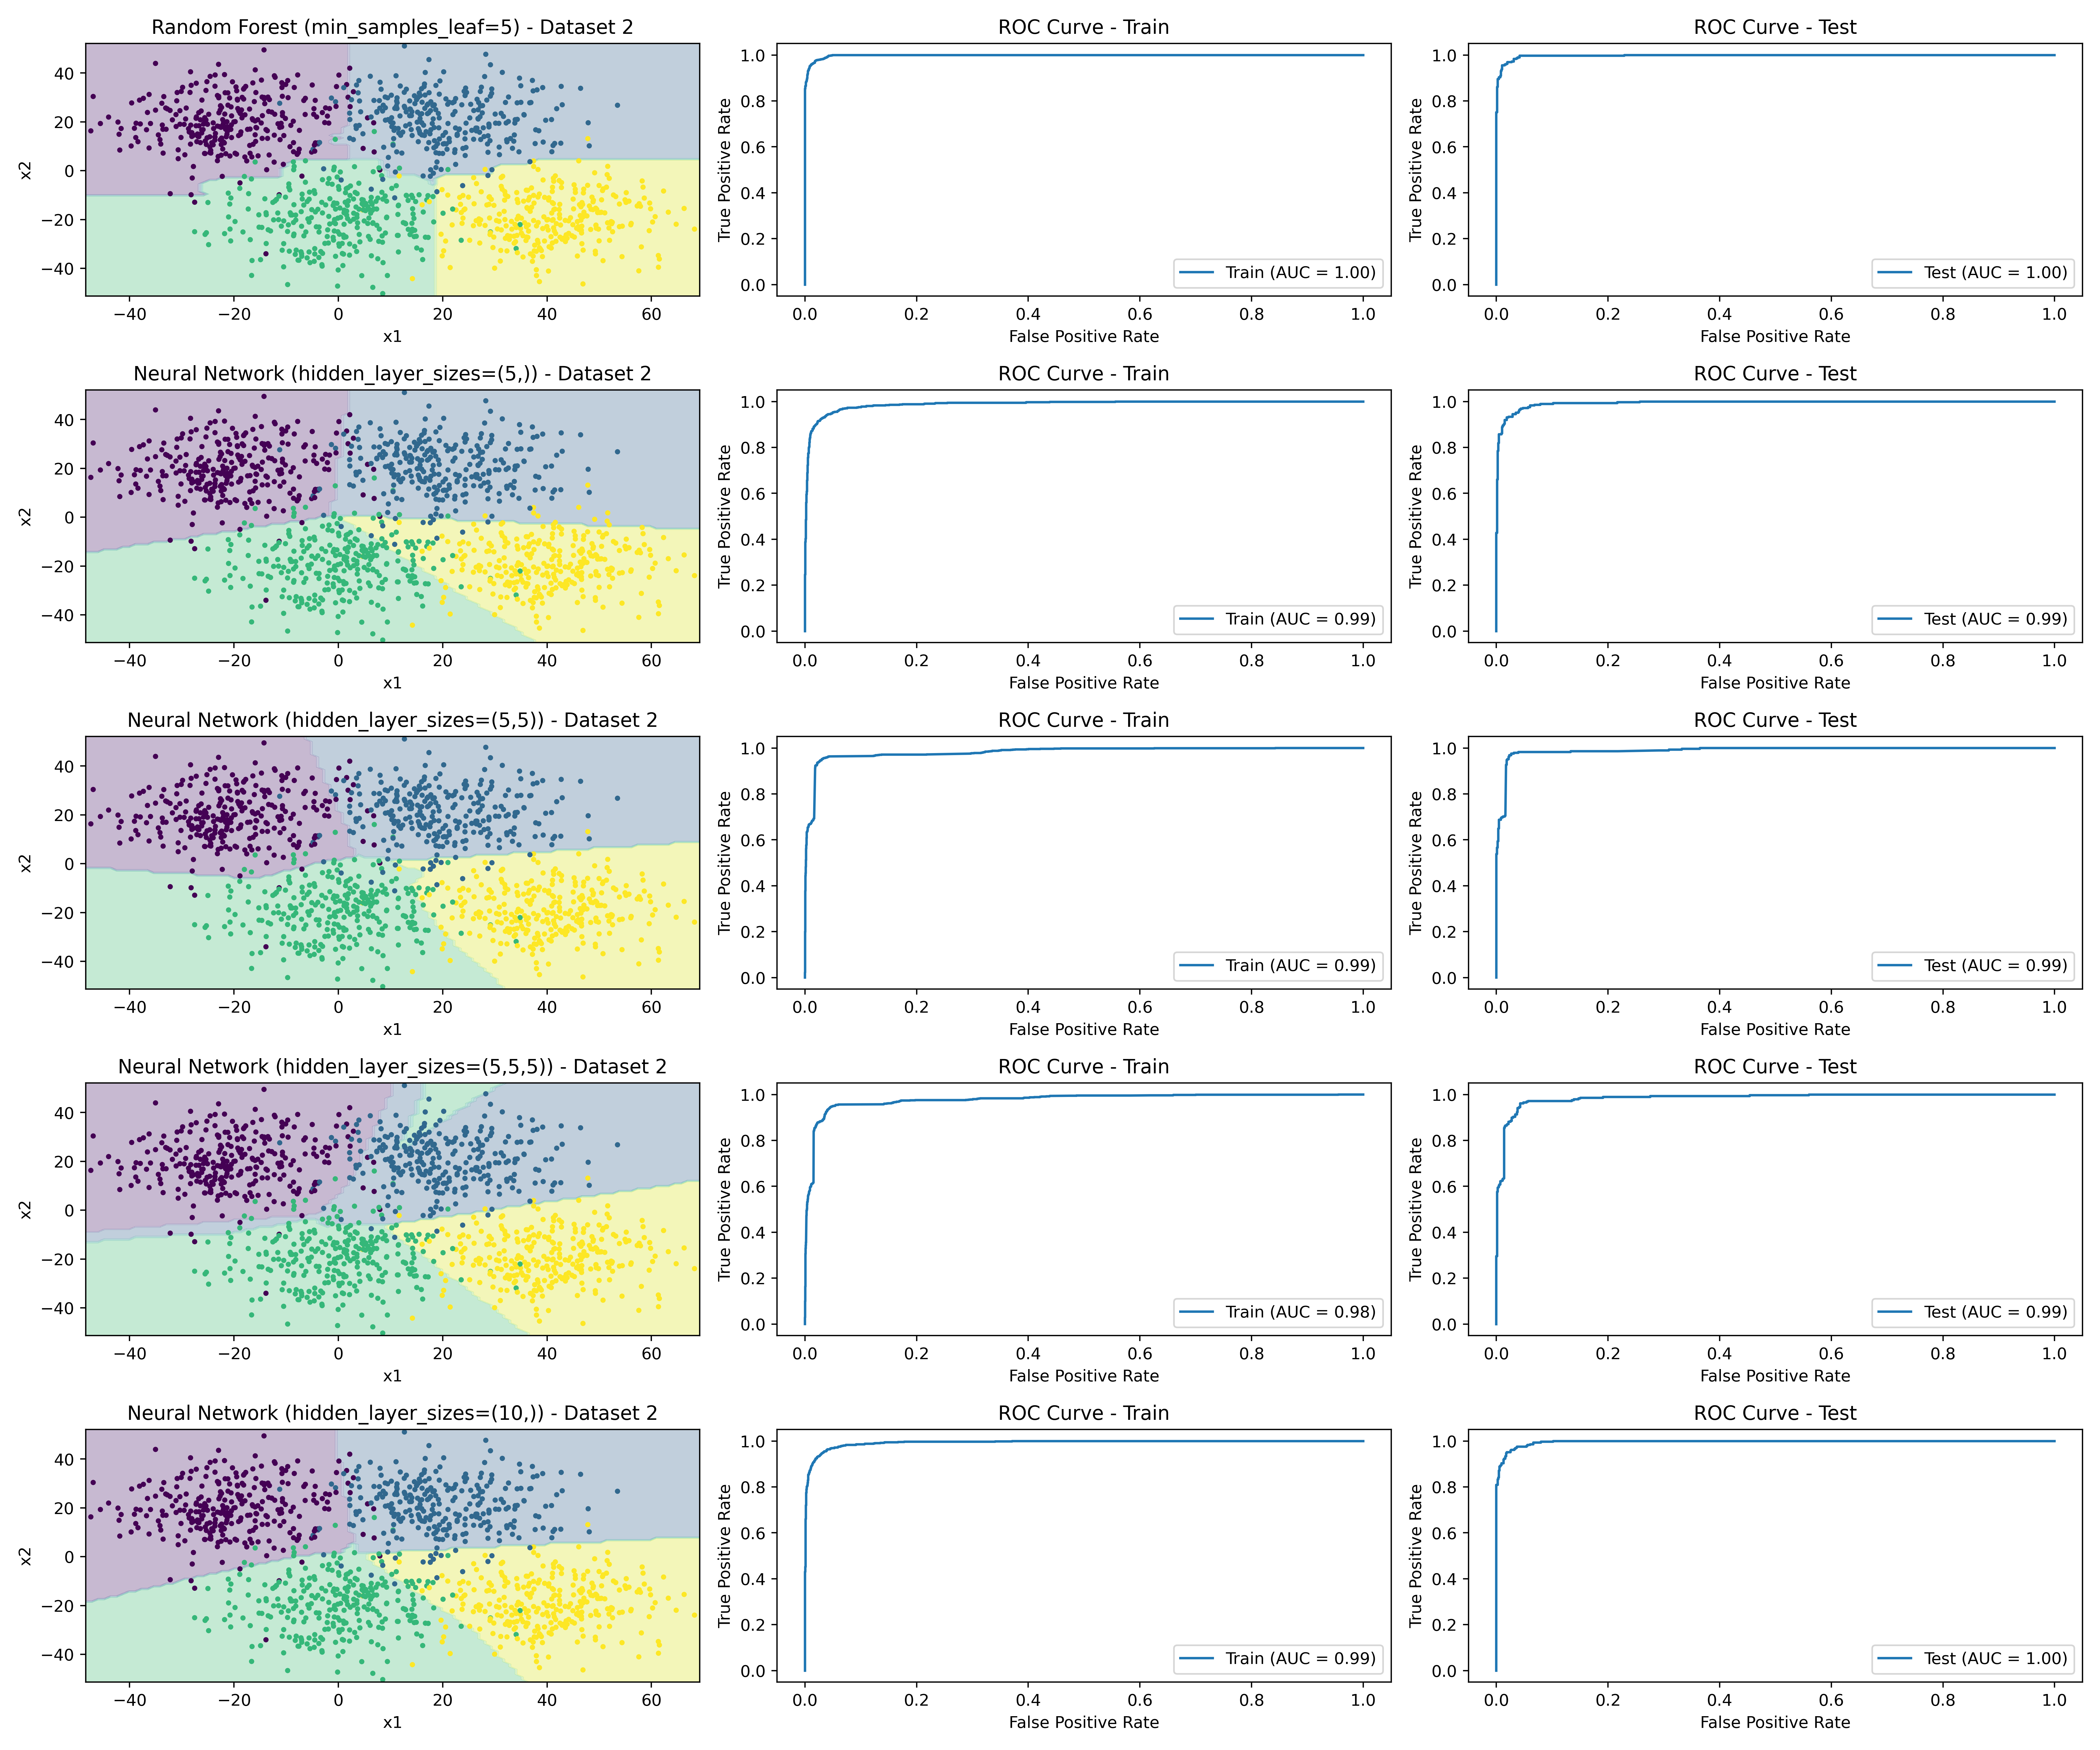
\includegraphics[width=\textwidth]{Images/dataset-2-roc-curves-2.png}
    \caption{ROC Curves for Dataset 2 (continued)}
\end{figure}

Here, we observe that the Decision Boundaries are different for each algorithm, and the AUC score for all of them are close to 1. For Neural Networks with \texttt{hidden\_ayer\_size=(5,)}, theh AUC Value drops to $0.97, 0.98$, but it is still close to 1. This indicates that all the algorithms are able to classify the data points in Dataset 2 with high accuracy.

The ROC Curves are also not ideal for all the algorithms, but they are close to the top-left corner of the plot. This shows us that the classifiers are able to distinguish between the positive and negative classes with high accuracy.

\begin{figure}[H]
    \centering
    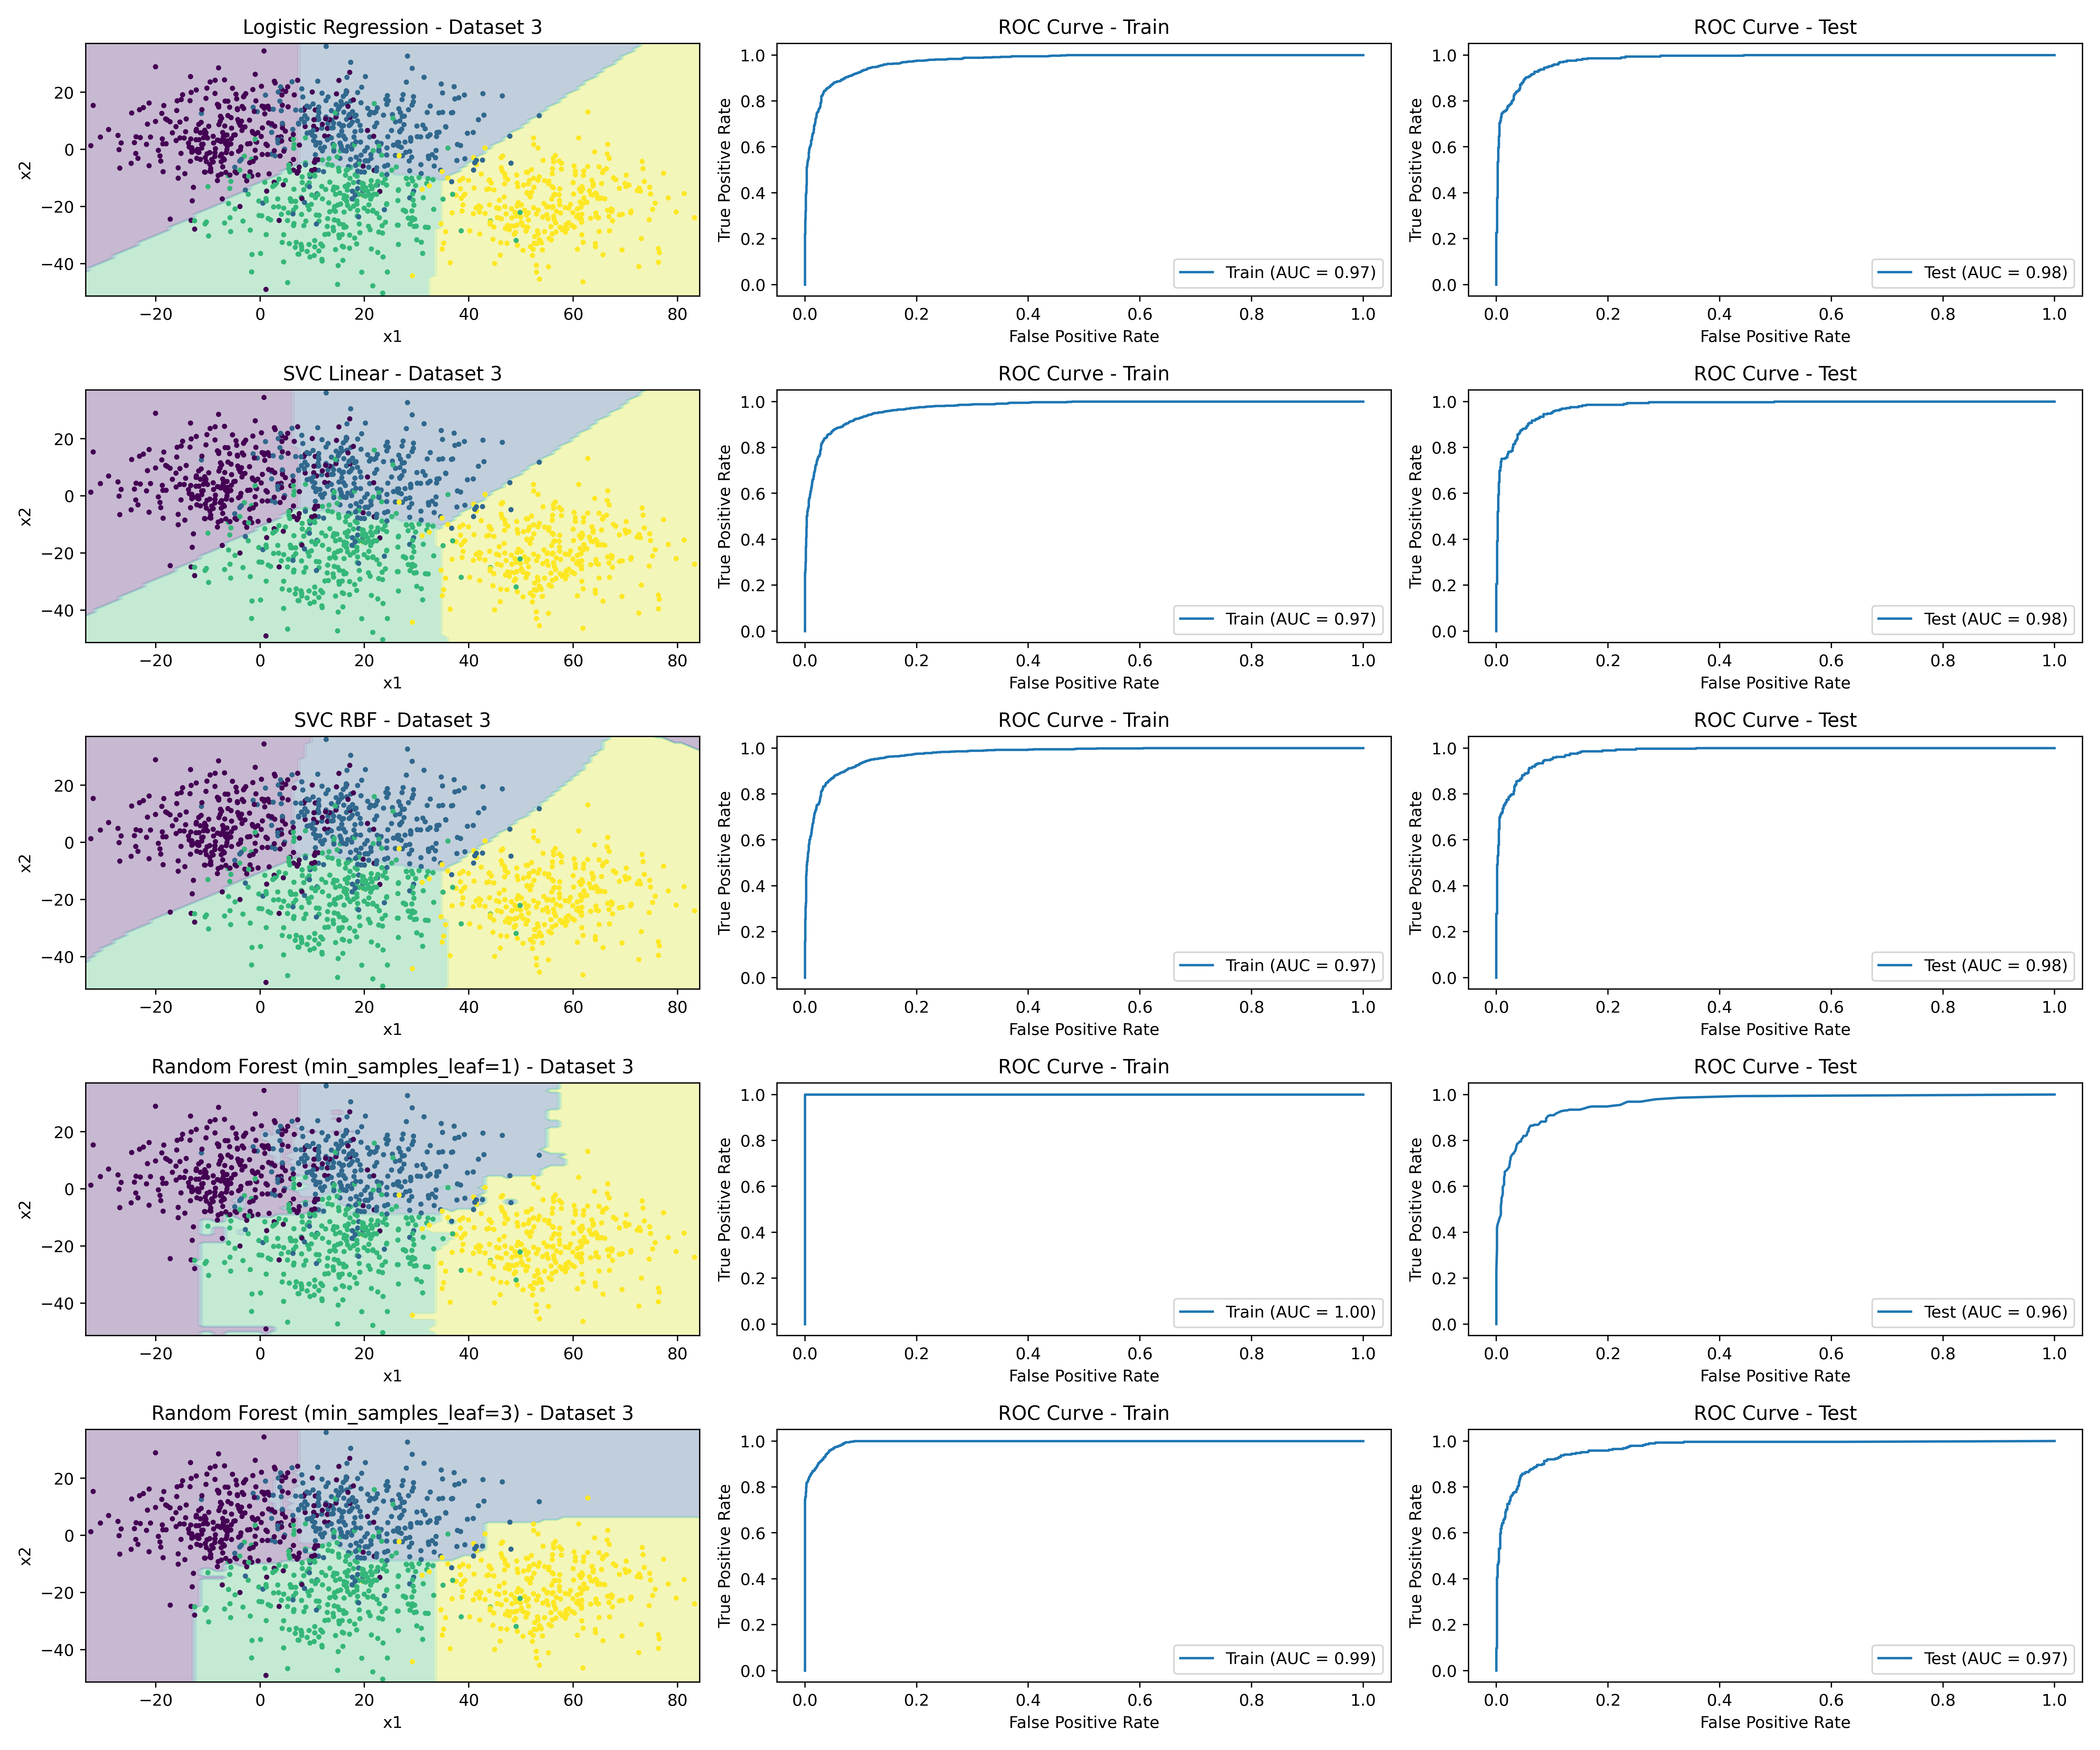
\includegraphics[width=\textwidth]{Images/dataset-3-roc-curves-1.png}
    \caption{ROC Curves for Dataset 3}
\end{figure}

Here, we observe that the Decision Boundaries are different for each algorithm, and the AUC score for all of them are lesser than the previous datasets. The AUC score for all the algorithms is still close to 1. This indicates that all the algorithms are  still able to classify the data points in Dataset 3 with high accuracy.

The ROC Curves are also not ideal for all the algorithms, but they are still above the diagonal line. This shows us that the classifiers are able to distinguish between the positive and negative classes with high accuracy.

\begin{figure}[H]
    \centering
    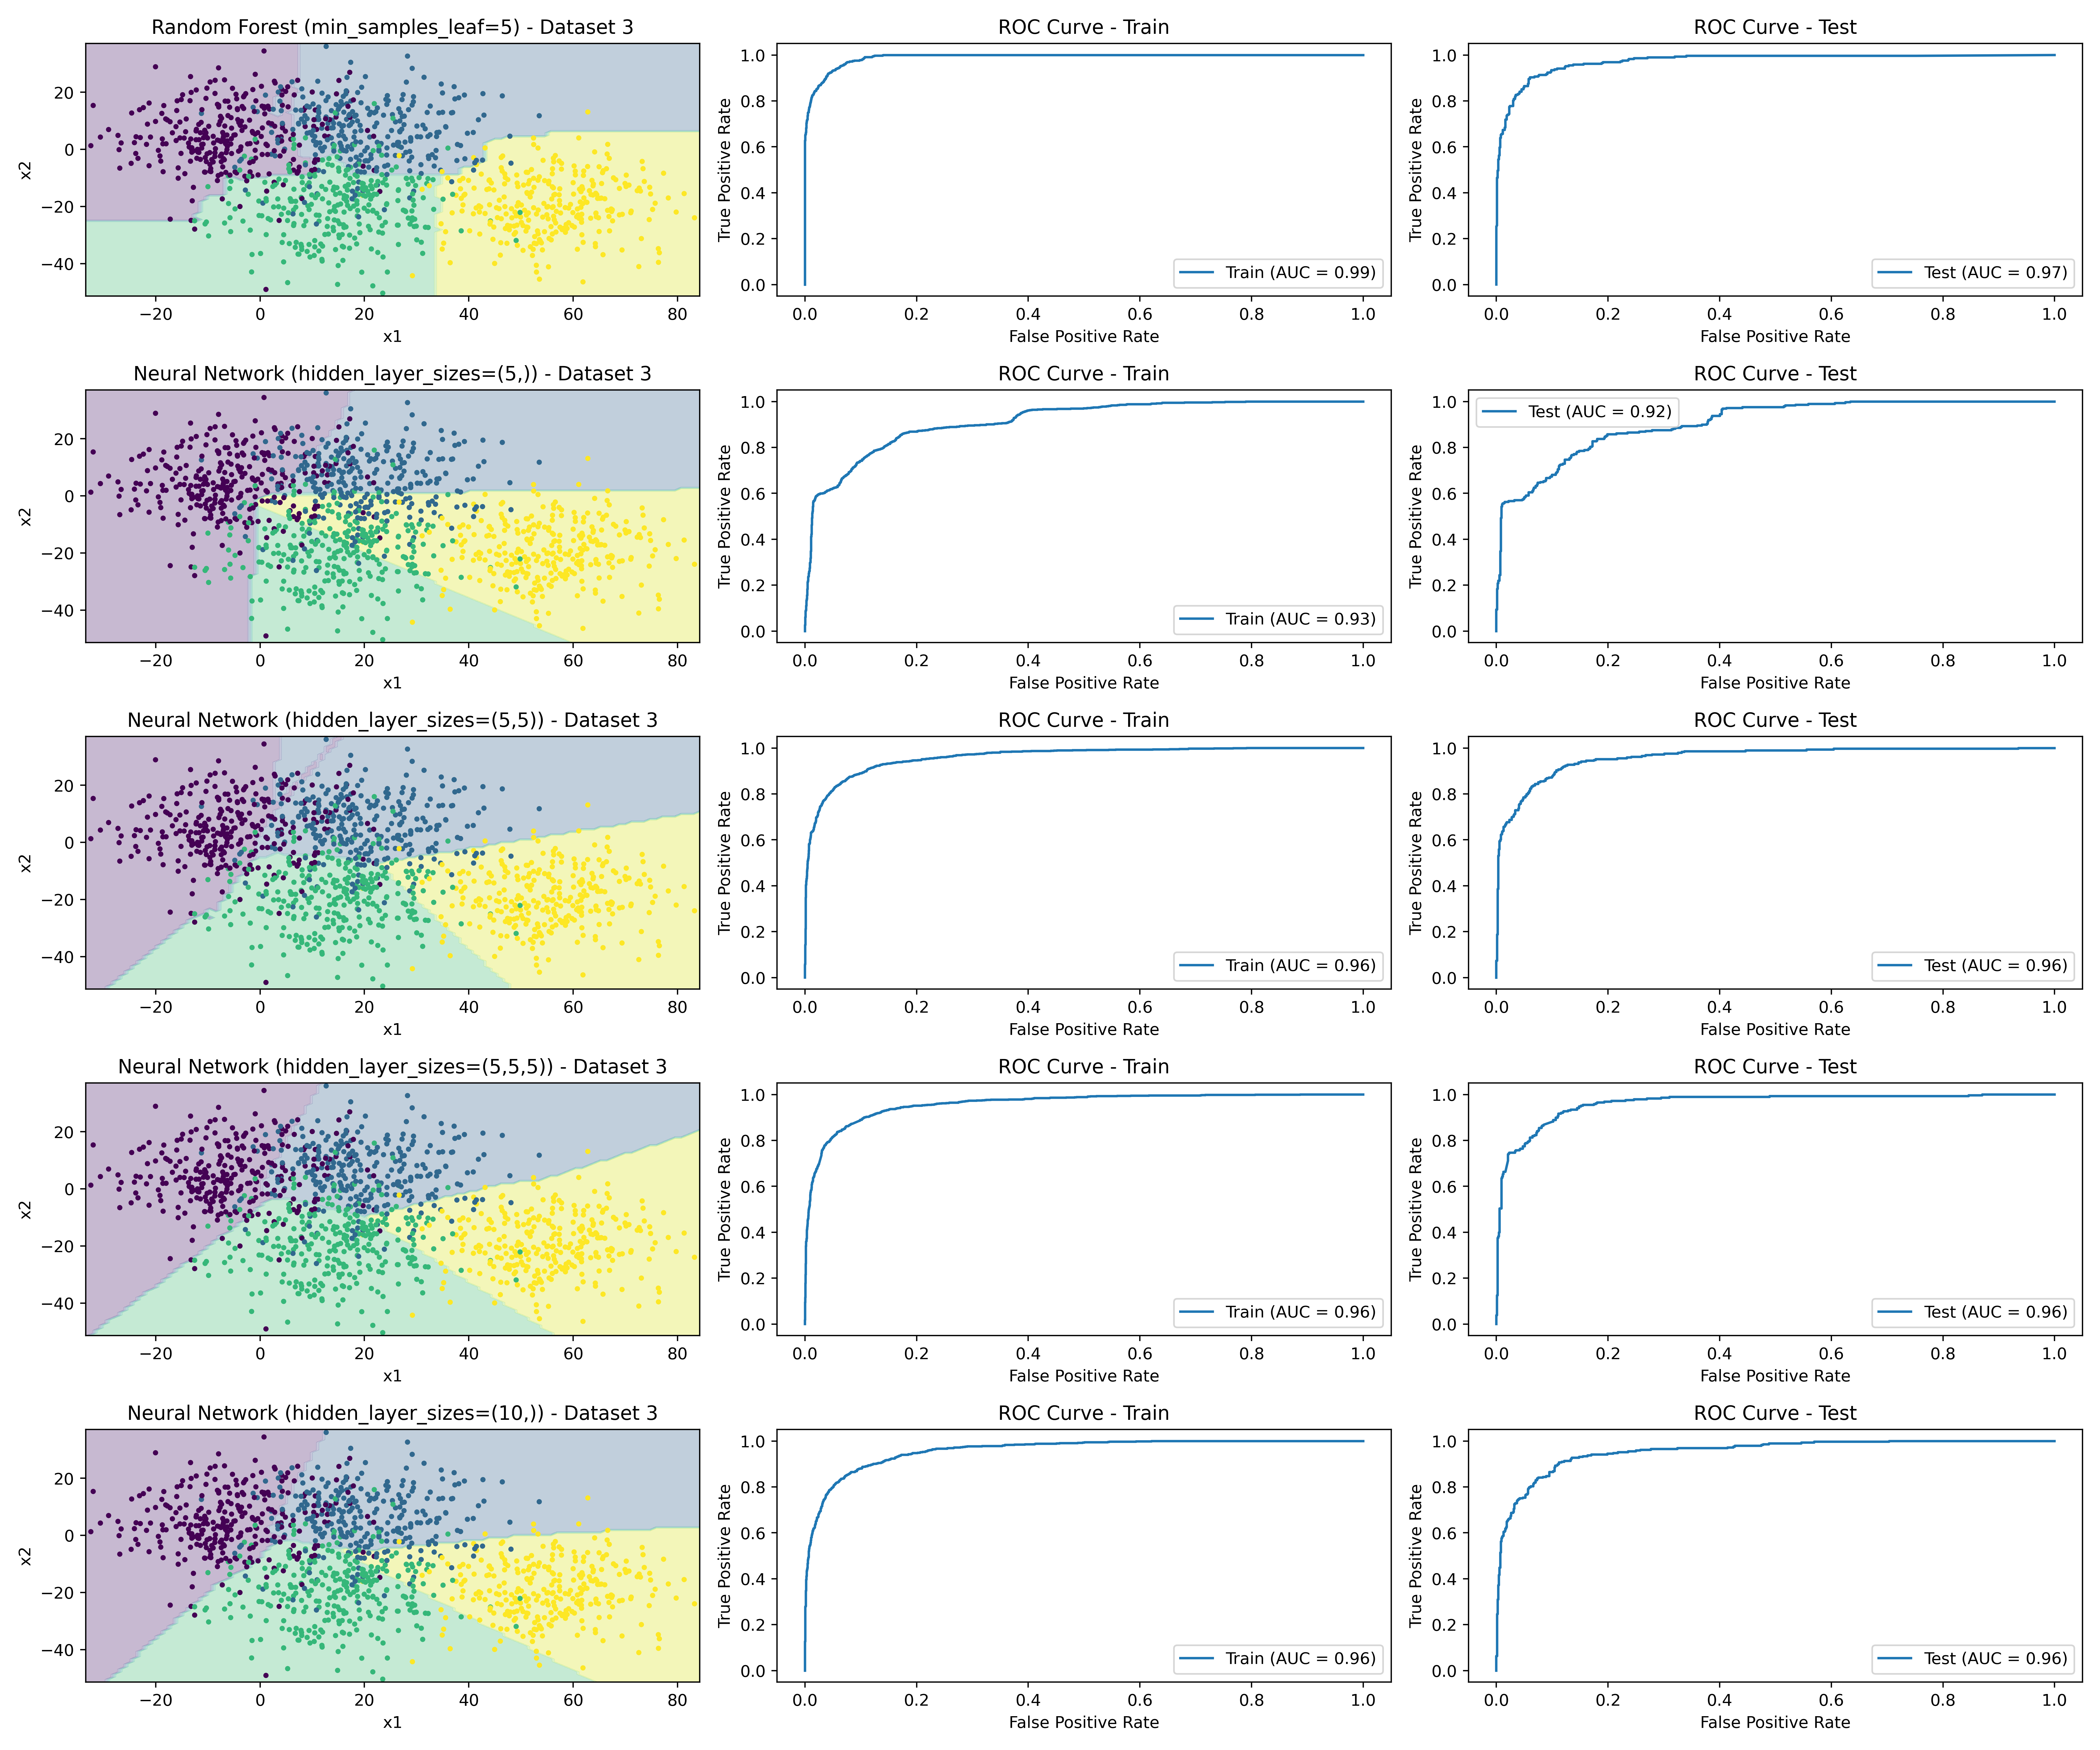
\includegraphics[width=\textwidth]{Images/dataset-3-roc-curves-2.png}
    \caption{ROC Curves for Dataset 3 (continued)}
\end{figure}

Here, we observe that the Decision Boundaries are different for each algorithm, and the AUC score for all of them are lesser than the previous datasets, with the least AUC score of $0.87, 0.86$ for Neural Networks with \texttt{hidden\_layer\_size=(5,)}. This indicates that all the algorithms are still able to classify the data points in Dataset 3 with good accuracy.

The ROC Curves are also not ideal for all the algorithms, but they are still above the diagonal line. This shows us that the classifiers are able to distinguish between the positive and negative classes with good accuracy.






